\begin{figure}[ht]
\centering
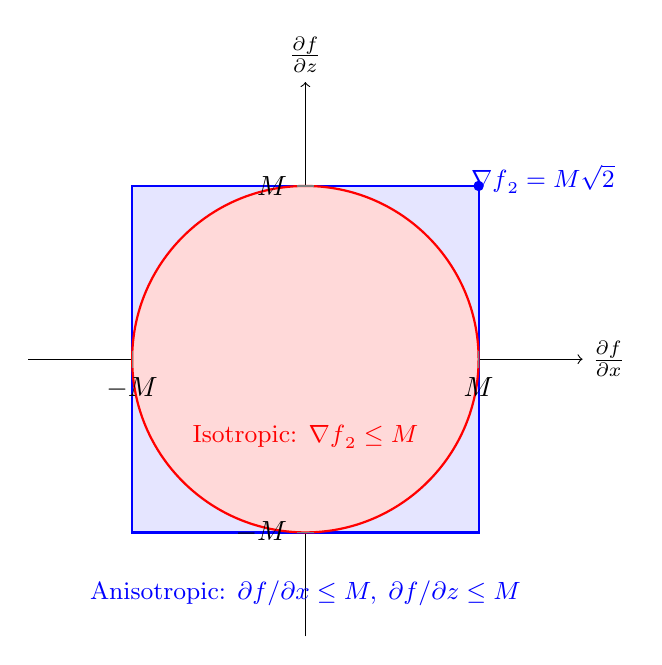
\begin{tikzpicture}[scale=2.2]
	% Axes
	\draw[->] (-1.6,0) -- (1.6,0) node[right] {$\frac{\partial f}{\partial x}$};
	\draw[->] (0,-1.6) -- (0,1.6) node[above] {$\frac{\partial f}{\partial z}$};

	% Anisotropic square (M_x = M_z = M)
	\fill[blue!10, draw=blue, thick]
		(-1,-1) rectangle (1,1);

	% Isotropic disk
	\fill[red!15, draw=red, thick]
		(0,0) circle (1);

	% Labels for M on axes
	\draw[thin, gray] (1,0.05) -- (1,-0.05) node[below, black] {$M$};
	\draw[thin, gray] (-1,0.05) -- (-1,-0.05) node[below, black] {$-M$};
	\draw[thin, gray] (0.05,1) -- (-0.05,1) node[left, black] {$M$};
	\draw[thin, gray] (0.05,-1) -- (-0.05,-1) node[left, black] {$-M$};

	% Corner point of square not in disk
	\fill[blue] (1,1) circle (0.03);
	\node[blue, above right, font=\small] at (0.9,0.9) {$\norm{\nabla f}_2 = M\sqrt{2}$};

	% Legend
	\node[red, font=\small] at (0, -0.45) {Isotropic: $\norm{\nabla f}_2 \leq M$};
	\node[blue, font=\small] at (0, -1.35) {Anisotropic: $\abs{\partial f/\partial x} \leq M,\; \abs{\partial f/\partial z} \leq M$};
\end{tikzpicture}
\caption{Feasible gradient sets for the isotropic and anisotropic Lipschitz classes with equal constants $M_x = M_z = M$.
The isotropic class constrains the gradient to lie in the disk (red); the anisotropic class constrains it to the square (blue).
The square strictly contains the disk: $\mathcal{F}_1^{\mathrm{iso}}(M) \subsetneq \mathcal{F}_1^{\mathrm{aniso}}(M, M)$.
At the corner $(M, M)$, the gradient magnitude is $M\sqrt{2}$, so a function with both partial derivatives at their bound lies in the anisotropic class but not the isotropic class.}
\label{fig:smoothness_classes}
\end{figure}
